\documentclass[a4paper,10pt]{article} 
\usepackage[margin=3.2cm]{geometry}
\usepackage{booktabs} 
\usepackage{graphicx} 
\usepackage{amssymb}
\usepackage{amsmath} 
\usepackage{xcolor}
\usepackage{setspace} 
\usepackage{natbib}
\usepackage{hyperref}
\usepackage{doi}
\usepackage{pdfpages}
 
\onehalfspacing

\newcommand{\revpoint}[3] 
{ \hrule ~\\[0.5em]
\noindent\textcolor{gray}{\noindent#1} \\[0.5em]  
\noindent\textcolor{blue}{\textit{\noindent#2}} \\[0.5em]
\noindent\textcolor{black}{\noindent{#3}} \\[0.5em]
}

\newcommand{\com}[1]{\textcolor{red}{\noindent#1}}


\title{Response to Reviewers} 
\author{Cedrick Ansorge and Hauke Wurps }
\begin{document}
\maketitle

%-------------------------------------------------------------------------------------%

%######################################################################################%
% not all comments are included, only where action is needed.
%######################################################################################%

\section*{Response to Reviewer 1}

Dear Reviewer 1, \\[1em]

\noindent Many thanks for the positive feedback on our manuscript. We have addressed the minor points raised in your review and hope that you agree with the edits. Pleas find the detailed responses below.  \\[1em]


\noindent Kind regards, \\[0.5em]

\noindent Cedrick Ansorge and Hauke Wurps  \\[0.5em]
%-------------------------------------------------------------------------------------%


\revpoint{The authors analyze wind speed and direction profiles in turbulent Ekman flow using asymptotic theory and DNS data. They found that the streamwise velocity follows classical scaling laws, while outer-layer profiles align with a modified Ekman spiral. They showed that the spanwise component exhibits mixed scaling near the surface and outer scaling farther out. \newline  Overall, the analysis and DNS are conducted rigorously, providing valuable insights and contributing meaningfully to advancements in the field.}{We sincerely thank you for the positive assessment of our manuscript and the appreciation of our work.}{}

\revpoint{In line 47, friction velocity is denoted as $u_* = \sqrt{|\tau_{sfc}/\rho}$. However, in Eq. (1a) (below line 179), $\tau_{sfc}$ is defined as the kinematic shear stress. Please make them consistent. }{Manz thanks for spotting this inconsistency in nomenclature. We have aligned $\tau_\text{sfc}$ with the conventional definition of dynamic shear stress and now include the division bz density in Eq. (1b).}{\begin{subequations}\begin{equation}
    \underline{\tau}_\mathrm{sfc} = \left(\begin{array}{c} \tau_x\\ \tau_y\\\tau_z\end{array}\right) = - \rho\nu \left( \frac{\partial U}{\partial z} \hat{e}_x + \frac{\partial V}{\partial z} \hat{e}_y\right)
  \end{equation}
  and labelled by an upper index $\alpha$ as in $\underline{U}^\alpha$ for the velocity vector, and
  (ii) the coordinate system aligned with the free-atmosphere geostrophic wind labelled by an upper index $G$ as in $\underline{U}^G$.
  %
  We denote the square root of the modulus of surface shear, the surface friction, by
  \begin{equation}
    u_\star = \sqrt{ \frac{|| - \underline{\tau}_\mathrm{sfc} ||}{\rho} } 
    \label{eqn:ustar_def}
  \end{equation} and let $Z_\star=G/u_\star$;
\end{subequations}}

\revpoint{Location for the definition of $z^-$. The first appearance of $z^-$ is at line 262, and figure 1b, but it was defined on line 307. It would be better to define it close to where it appears. }{Thank you - we now introduce the outer length scale much earlier in Sec. 2.1 ("Notation and governing equations"). We also think, this is more appropriate.}{The outer normalization (with respect to the boundary-layer depth $\delta$ and velocity $u_\star$) is denoted 
by a superscript $'-'$, i.e. $z^-=z/\delta$.  }

\revpoint{Figure 4: Should the legend be $Z_* = 4 log(Re_D) -8$, instead of $u_\star* = ...$"?}{Indeed, there was a typo, please find the revised Figure below.}{
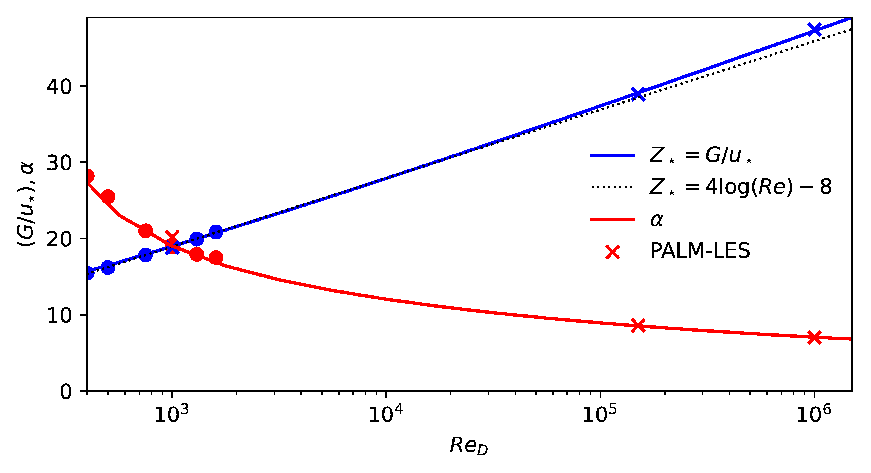
\includegraphics[width=\textwidth]{Fig4.eps}
}
\newpage
\section*{Response to Reviewer 2}
\revpoint{The authors perform direct numerical simulations of the Ekman layer at moderate Reynolds number, and use their simulations to examine the vertical mean velocity profiles in rotating, neutrally-stratified flows that serve as a proxy for the neutral atmospheric boundary layer. They compare their DNS results to a model that matches the Ekman model (in the outer layer) with the classical results for the inner layer (viscous layer plus log layer) in wall-bounded turbulent flows. Specifically, they examine the scaling of the spanwise velocity profile, and find that a matching procedure—combining both inner- and outer-scaling—is necessary. The article is generally clear and well-written, and addresses the important problem of how velocity profiles behave in the Ekman layer. Despite being an old problem, it has not been resolved, and there are many subtleties that are often neglected in the literature. I am overall supportive of this manuscript, but below I provide some specific comments which I believe will help improve the clarity of communication in the article. I am recommending that the manuscript is accepted in BLM, pending minor revisions. }{We appreciate your summary of our work and thank you for the time spent on our manuscript. Below, please find the detailed responses to your comments.}{}

\revpoint{L. 12, 76: discussion of span-wise velocity component. Can you explain how you are defining streamwise and spanwise here? Are you assuming the streamwise component is aligned with the geostrophic wind direction far above the surface? }{This is indeed important and we inserted an apposition phrase for clarification}{[\ldots], considered in a wall-stress-aligned reference frame, [\ldots]}

\revpoint{L. 16 outer height - do you mean outer length scale? }{We mean 'outer height' here, but we realize the phrase may be uncommon to some BLM readers and have clarified as follows}{[\ldots] commonly denoted as $z^-$.}

\revpoint{L. 19 “vide Reynolds numbers” - I’m not sure this makes sense to me. }{What we mean here is that an 
increase in scale separation is the same as an increase in Reynolds number. We rephrased}{[\ldots], i.e. an increase in Reynolds number.}

\revpoint{L. 63 Prandtl-layer height is undefined here}{The symbol was superfluous and is not needed. We now describe what the Prandtl-layer height is and trust that the interested reader will be able to find details on the exact definition in the reference that is mentioned here. }{[\ldots] they choose the Prandtl-layer depth, a measure for the depth of the surface layer, to match the wind speed profiles. 
However, this requires external prescription of the veering at that height. }

\revpoint{L. 124 - “require one to consider” or “require consideration of” }{Thank you! We chose the latter.}{[\ldots] require consideration of the height-dependence of the veer and stress misalignment [\ldots].}

\revpoint{ll. 168-170 - This seems to be contradictory. The authors state that rotation only acts on the horizontal components of velocity, but go on to state that they neglect rotational effects on the horizontal components of velocity. }{Thank you for spotting this inconsistency, of course rotational effects on the \textbf{horizontal} components of velocity are considered, they are only neglected for the \textbf{vertical} components. }{The f-plane approximation is applied, i.e. rotation acts on the horizontal components of velocity alone; rotational effects on the vertical component of velocity and dynamical effects
due to latitudinal variation of the rate of rotation are neglected.}

\revpoint{l. 176 - I do not think that Ensemble should be capitalized }{adopted.}{}

\revpoint{L. 193 “this state is defined by a Reynolds number, the only non-dimensional parameter that governs the system.” Shouldn’t the Rossby number also enter as a non-dimensional parameter? Given a domain height, geostrophic wind speed G, and Coriolis parameter f, one can also define the Rossby number. The problem would depend on Reynolds number alone in the absence of rotation, but if there is rotation, the relevant dimensionless parameters should be both Re and Ro. }{In general, this is true. However, when Ekman flow is considered, the ratio of Rossby and Reynolds number (which is the Ekman number) is fixed. To clarify the impact of this constraint: it also implies that - given the Coriolis parameter $f$, i.e. a latitude - the geostrophic wind defines the Rossby radius. That is, Ekman flow is  a rather strong constraint form the perspective of large-scale dynamics. Nonetheless, it is a widely adopted simplification in the context of boundary-layer dynamics. We add a phrase clarifying the uniqueness of the problem given $Re$. For clarification, one may see that the Ekman-based Reynolds number $Re_D$ can be written as Ratio of the Rossby Radius $\Lambda_\text{Ro}$ and laminar Ekman-layer scale $D$, which is another illustration of the link between large-scale and boundary-layer dynamics: \begin{equation} Re_D = \frac{GD}{\nu} = \frac{G \sqrt{2\nu}}{\sqrt{f}\nu}= \sqrt{\frac{2 G^2}{f\nu}}=\sqrt{\frac{G^2}{f^2}\frac{2f}{\nu}}=\sqrt{4 \Lambda_\text{Ro}^{2} \frac{f}{2\nu}}=2\Lambda_\text{Ro}/D.\label{eqn:re-relation}\end{equation}
Analogously, one may see that 
$Ro = \frac{G}{\Lambda_\text{Ro}f} = 1$ for the definition of the Rossby number. Alternatively -- when replacing $\Lambda_\text{Ro}$ by $D$, which also yields a valid definition of Rossby number from the perspective of boundary-layer dynamics-- it is (cf. Eq.~\ref{eqn:re-relation})
\begin{equation}
\text{Ro}_D=\frac{G}{Df} = \text{Ro} \frac{ D}{\Lambda_\text{Ro}} = \frac{2}{Re_D}
\end{equation} 
}{}

\revpoint{L. 221 - It might be better to use scientific notation here. }{As we do need five significant digits for the middle number, we do not see the benefit of moving to scientific notation}{ // no change incurred //}

\revpoint{L. 277, 281 - the notation is a bit awkward here, e.g. $V^{\alpha_\star+}(z^+)$. Is there a way to make it clearer? }{We have thought a lot about this notation and checked many different approaches. It is very important to note that the index $a_\star$ cannot simply ommited (in fact, above it has been demanded to clarify the alignment, which is the sole purpose of the index $\alpha_\star$). At the moment, we do not see a better option - if there may be more aesthetic options, all of them which come to our mind, would sacrifize clarity.}{// no change incurred // }
\revpoint{Fig. 1a - Does the solid black line correspond to the Re=1600 case? If so, why is there i a discontinuity just above $10^1$? Or are you also using a solid black line to denote the inner layer velocity profile, $u^+ = z^+$? }{}{}
\revpoint{L. 308 Eddy should not be capitalized}{adopted}{The eddy viscosity [\ldots]. }
\revpoint{L. 311 - The assumptions of horizontal homogeneity and W=0 are not exactly the same thing as symmetries in the flow. }{We realize that this was an imprecise phrasing and clarified.}{For the assumptions of horizontal homogeneity and incompressibility (which implies  $W=0$, i.e. no mean wall-normal velocity), it is [\ldots].
}
\revpoint{Fig. 3: It would be better to present heights in terms of $z^+$ values rather than the index of the vertical coordinate. }{We believe that both ways of conveying this information have their value and added the requested distance from the wall in inner units.}{\textbf{Fig.\,3\ }Horizontal slices of turbulence kinetic energy in the
Buffer layer (i=10, $z^+\approx 10.5$),
logarithmic layer (i=100, $z^+ \approx 150$), and
outer layer (i=400, $z^+ \approx 1200$) of the case with $Re_\tau=2978$;
coloring between percentiles 4 and 96 of the respective image. Lower panel:streamwise--vertical intersect through the domain 
\label{fig:slices}} 


\newpage
\section*{Response to Reviewer 3 (Prof. Sukanta Basu)}

Dear Professor Basu, \\[1em]

\noindent we like to extend our sincere thanks for your assessment of our manuscript. We understand your criticism of our somewhat bold claim of universality and have amended the manuscript.\\[1em]

\noindent We ask for your understanding that, as you already anticipated, a complete reconsideration of our results in the framework of your 2023 paper is not carried out at this point. We, however, would be happy to provide processed and unprocessed data if a colleague or potentially member of your working group is interested in carrying these ideas further.\\[1em]

\noindent As you unveiled your identity and you gave your consent to be mentioned, we also thank for your contribution in the acknowledgments of the revised manuscript. \\[1em] 

\noindent Cedrick Ansorge and Hauke Wurps \\[2em]
\hrule


\revpoint{This is an excellent paper that should be published in BLM. However, I request the authors to tone
down their narrative, including the title. It is an empirical study that tries to fit DNS data using various
formulations. Some of these formulations have a physical basis, while others are ad-hoc. Please refrain
from calling the results “universal”. }{We critically reassessed our use of the work 'universal' in the manuscript and indeed agree that in some respect, in particular with respect to the derived velocity-profile formulations the use was somewhat overstating. We removed these occurrences in the introduction, conclusion and some parts of the results. Most importantly, we removed the word from the running title and from the section title. However, in the context of some the classic universal scalings *(logarithmic scaling, viscous scaling), we keep the word -- also in the context of our results.}{A number of changes was carried out throughout the manuscript in response to this point, we kindly ask you to refer to the annotated pdf file for deatils. Primarily we undertook the following modifications \\
  (1) changed title to \textbf{Wind veer and speed in turbulent Ekman flow part I: scaling analysis and velocity profile model}\\
  (2) changed heading of Section 4.1 to \textbf{A Reynolds-number-independent velocity profile for the turbulent Ekman layer}\\
  (3) Conclusions: universal formulation $\rightarrow$ \textbf{closed formulation} } 


\revpoint{At the heart of this paper is Eq.~10a. Following Etling's work and others, this equation has been derived in Appendix A1. \newline 
  \[
    \frac{1}{G} \left(\begin{array}{c}U_\text{Ek} \\ V_\text{Ek} \end{array}\right) = \left(\begin{array}{c} 1 \\0 \end{array}\right) + e^{-z_\text{Ek}} \left[ a_\text{ek} \left(\begin{array}{c} -\cos z_\text{ek} \\ \sin z_\text{ek} \end{array}\right)+ b_\text{ek}\left(\begin{array}{c}\sin z_\text{ek} \\ \cos z_\text{ek}\end{array}\right)   \right]
  \] \newline  
  The problem with this equation is the assumption of constant eddy viscosity. As the authors showed in
  Figure 2c, the eddy viscosity profile from the DNS is far from constant. It has a clear maximum and a
  specific shape, which depends on Re.
  So, the authors took an empirical (engineering) approach on page 14 (line 403). They estimated a bulk
  eddy viscosity indirectly. This is a major weakness of this paper and could be avoided. Please see the
  following paper where we analytically derived the eddy viscosity profile from the Ekman equations.
  Since this is a relatively new paper, the authors might not have come across it. That is why I am revealing
  my identity.
  \begin{quotation}Basu, Sukanta, and Albert AM Holtslag. “A novel approach for deriving the stable
  boundary layer height and eddy viscosity profiles from the Ekman
  equations.” Boundary-Layer Meteorology 187.1 (2023): 105-115.
  \end{quotation}
  The authors might want to revise their derivations based on our analytical eddy viscosity profile. If that
  is difficult to do, I suggest highlighting the limitations of their current bulk approach. Also, emphasize
  the limitations of Eq. (10a) as it assumes constant eddy viscosity. }{}{}

\revpoint{Could the authors comment on Fig. 6a in the revised manuscript? The discrepancy between DNS and
  their empirical prediction is large and not explained.
}{}{}
\end{document} 